%!TEX root = ../thesis.tex
%*******************************************************************************
%****************************** Third Chapter **********************************
%*******************************************************************************
\chapter{Bispectrum and Primordial Non-Gaussianity}

% **************************** Define Graphics Path **************************
\ifpdf
    \graphicspath{{Chapter3/Figs/Raster/}{Chapter3/Figs/PDF/}{Chapter3/Figs/}}
\else
    \graphicspath{{Chapter3/Figs/Vector/}{Chapter3/Figs/}}
\fi

The primordial perturbations are consistent with being Gaussian distributed according to observations \cite{PlanckCollaboration2018}. Statistical properties of a Gaussian random field are completely characterised by its mean and covariance functions. Since CMB is a near-linear probe of the early universe, its power spectrum directly relates to covariance functions of the initial fluctuations. CMB power spectrum is a sufficient statistic in the perfect Gaussian limit, which means that it contains all the information about initial conditions we may ever extract from CMB. The inverse is also true however; if the initial conditions are non-Gaussian, it is essential to go beyond the power spectra and study higher-order statistics. Such non-Gaussian contributions are best captured in three-point correlation functions, or their Fourier counterpart: bispectrum.

In a single field slow-roll inflation with standard kinetic term and vacuum, the primordial bispectrum is suppressed by slow-roll parameters \cite{Maldacena2013}. Numerous other inflationary scenarios that are physically well-motivated violate these simple assumptions and hence predict non-Gaussian signatures. They are expected to leave imprints on CMB bispectrum with characteristic shape and amplitude, where the latter is parametrised by $f_{NL}$.

We discuss the bispectrum in relation to primordial non-Gaussianity in this section, from both theoretical and observational side. Section \ref{section:bispectrum} covers the basic formalism of bispectrum analysis. Section \ref{section:primordial_non_Gaussianity} then introduces theoretical tools for calculating the primordial bispectrum from a given inflation model Lagrangian. On the CMB side, we formulate the optimal bispectrum estimator and existing implementations of it in Section \ref{section:CMB_bispectrum_estimation}.


\section{Bispectrum} \label{section:bispectrum}

Consider the three-point correlation function $\left< \zeta(\vv{x}_1) \zeta(\vv{x}_2) \zeta(\vv{x}_3) \right>$  of the curvature perturbation $\zeta$ at the end of inflation. Its Fourier transform is given by
\begin{align}
	\left< \zeta(\vv{k}_1) \zeta(\vv{k}_2) \zeta(\vv{k}_3) \right> = \int d^3\vv{x}_1 d^3\vv{x}_2 d^3\vv{x}_3 \; e^{-i(\vv{k}_1 \cdot \vv{x}_1 + \vv{k}_2 \cdot \vv{x}_2 + \vv{k}_3 \cdot \vv{x}_3 )} \left< \zeta(\vv{x}_1) \zeta(\vv{x}_2) \zeta(\vv{x}_3) \right>. \label{eqn:bispectrum_from_fourier_derivation_1}
\end{align}
Statistical homogeneity implies that correlation functions are invariant under spatial translation $\vv{x} \rightarrow \vv{x}' = \vv{x} + \vv{c}$. In particular, we have $\left< \zeta(\vv{x}_1) \zeta(\vv{x}_2) \zeta(\vv{x}_3) \right> = \left< \zeta(\vv{x}_1 - \vv{x}_3) \zeta(\vv{x}_2 - \vv{x}_3) \zeta(\vv{0}) \right>$. Relabelling the integration variables so that $\vv{x}'_1=\vv{x}_1-\vv{x}_3$ and $\vv{x}'_2=\vv{x}_2-\vv{x}_3$, \eqref{eqn:bispectrum_from_fourier_derivation_1} becomes
\begin{align}
	&\int d^3\vv{x}'_1 d^3\vv{x}'_2 d^3\vv{x}_3 \; e^{-i[ \vv{k}_1 \cdot (\vv{x}'_1 + \vv{x}_3) + \vv{k}_2 \cdot (\vv{x}'_2 + \vv{x}_3) + \vv{k}_3 \cdot \vv{x}_3 ]} \left< \zeta(\vv{x}'_1) \zeta(\vv{x}'_2) \zeta(\vv{0}) \right> \nonumber \\
	&\hspace{0.05\textwidth} = (2\pi)^3 \delta^{(3)}(\vv{k}_1 + \vv{k}_2 + \vv{k}_3) \int d^3\vv{x}'_1 d^3\vv{x}'_2 \; e^{-i( \vv{k}_1 \cdot \vv{x}'_1 + \vv{k}_2 \cdot \vv{x}'_2)} \left< \zeta(\vv{x}'_1) \zeta(\vv{x}'_2) \zeta(\vv{0}) \right> \label{eqn:bispectrum_from_fourier_derivation_2}\\
	&\hspace{0.05\textwidth} =: (2\pi)^3 \delta^{(3)}(\vv{k}_1 + \vv{k}_2 + \vv{k}_3) \; B(\vv{k_1}, \vv{k_2}), \label{eqn:bispectrum_from_fourier_derivation_3}
\end{align}
where we defined $B(\vv{k_1}, \vv{k_2})$ to be the integral expression appearing in \eqref{eqn:bispectrum_from_fourier_derivation_2}. The delta function enforces $\vv{k}_1 + \vv{k}_2 + \vv{k}_3 = \vv{0}$, which corresponds to conservation of momentum.

We now make use of statistical isotropy. Correlators remain constant under the rotation $\vv{x} \rightarrow \vv{x}' = R \vv{x}$ for any orthogonal matrix $R$. It is straightforward to see that $B(\vv{k}_1,\vv{k}_2)$ remains invariant under rotations as well;
\begin{align}
	B(R\vv{k}_1, R\vv{k}_2) &= \int d^3\vv{x}'_1 d^3\vv{x}'_2 \; e^{-i[ (R\vv{k}_1) \cdot \vv{x}'_1 + (R\vv{k}_2) \cdot \vv{x}'_2]} \left< \zeta(\vv{x}'_1) \zeta(\vv{x}'_2) \zeta(\vv{0}) \right> \\
	&= \int d^3\vv{x}''_1 d^3\vv{x}''_2 \; e^{-i( \vv{k}_1 \cdot \vv{x}''_1 + \vv{k}_2 \cdot \vv{x}''_2)} \left< \zeta(R \vv{x}''_1) \zeta(R \vv{x}''_2) \zeta(\vv{0}) \right> \;\;= B(\vv{k}_1, \vv{k}_2),
\end{align}
where we used the fact that $R^T=R^{-1}$. We may therefore fix $\vv{k}_1$ to be aligned with the $z$-axis, for example, and rotate further to have $\vv{k}_2$ lie in the $xz$ plane. $B$ therefore depends only on three variables: two lengths $k_1$, $k_2$, and an angle $\vv{k}_1 \cdot \vv{k}_2 / (k_1 k_2)$. Since $\| \vv{k_3} \|^2 = \| \vv{k}_1+\vv{k}_2 \|^2 = k_1^2 + k_2^2 + 2(\vv{k_1}\cdot\vv{k_2})$, the angle can be replaced by $k_3$. Putting everything together, we obtain
\begin{align}
	\left< \zeta(\vv{k}_1) \zeta(\vv{k}_2) \zeta(\vv{k}_3) \right> =  (2\pi)^3 \delta^{(3)}(\vv{k}_1 + \vv{k}_2 + \vv{k}_3) \; B(k_1, k_2, k_3).
\end{align}
Note that the bispectrum $B(k_1,k_2,k_3)$ is a three-dimensional function, as opposed to the one-dimensional power spectrum $P(k)$. The domain of $B$ is further restricted by the constraint that $k_1,k_2,k_3$ must form a triangle, which comes from the delta function.

The functional form of bispectrum comprises two parts: its dependence on the overall scaling $K=k_1+k_2+k_3$, called \textit{running}, and the \textit{shape} of the triangle formed by $k_1$,$k_2$ and $k_3$. Some notable shapes are depicted in Figure \ref{fig:triangle_configurations}.

\begin{figure}
	\centering
	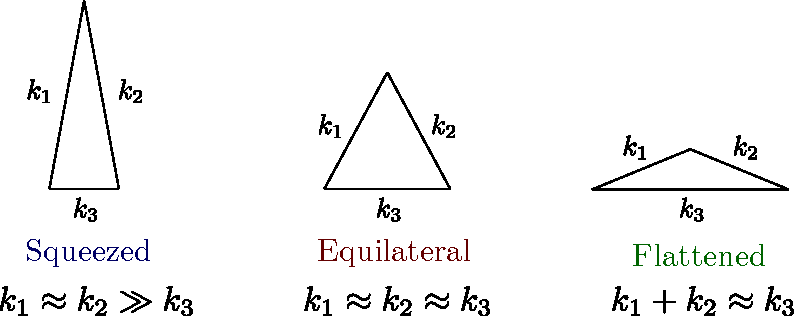
\includegraphics[width=0.8\textwidth]{triangle_configurations.pdf}
	\hspace{10pt}
	\caption{Three notable triangle configurations for the bispectrum $B(k_1,k_2,k_3)$.}
	\label{fig:triangle_configurations}
\end{figure}

The squeezed, equilateral and flattened limits of bispectra have distinct physical meaning. For example, the squeezed limit corresponds to a configuration with two small-scale (large $k$) modes and one large-scale (small $k$) mode. Heuristically, this relates to how small scale covariances are affected by an encompassing large scale mode.

One of the most studied shape of bispectrum arises from the \textit{local} model. In this model, the perturbative field $\zeta(\vv{x})$ is expanded as a local function of some Gaussian field $\zeta_G(\vv{x})$ as
\begin{align}
	\zeta(\vv{x}) = \zeta_G(\vv{x}) + \frac{3}{5} f_{NL} \left(\zeta_G^2(\vv{x}) - \left< \zeta_G^2 \right> \right) + \cdots. \label{eqn:local_model_fNL_defitintion}
\end{align}
The non-linearity parameter $f_{NL}$ measures the amplitude of quadratic contribution to the field. A factor of $(3/5)$ here comes from a convention; the original definition of $f_{NL}$ in terms of the potential $\Phi$, which is equal to $(3/5)\zeta$ on superhorizon scales.

Substituting this form into \eqref{eqn:bispectrum_from_fourier_derivation_1} gives correlation functions involving 4 Gaussian fields, to leading order in $f_{NL}$. Isserlis' theorem allows us to express such four-point correlators into sums of all possible contractions:
\begin{align}
	\left< \zeta_G(\vv{x}_1)^2 \zeta_G(\vv{x}_2) \zeta_G(\vv{x}_3) \right> = &\left< \zeta_G(\vv{x}_1)^2 \right> \left< \zeta_G(\vv{x}_2) \zeta_G(\vv{x}_3) \right> + \left< \zeta_G(\vv{x}_1) \zeta_G(\vv{x}_2) \right> \left< \zeta_G(\vv{x}_1) \zeta_G(\vv{x}_3) \right> \nonumber \\ &\hspace{0.15\textwidth} + \left< \zeta_G(\vv{x}_1) \zeta_G(\vv{x}_3) \right> \left< \zeta_G(\vv{x}_1) \zeta_G(\vv{x}_2) \right>. \label{eqn:local_model_derivation_1}
\end{align}
Contributions from the first term in \eqref{eqn:local_model_derivation_1} cancels out with ones coming from $\left< \zeta_G^2 \right>$ in the definition \eqref{eqn:local_model_fNL_defitintion}. Expressing two-point correlations in terms of power spectrum in Fourier space, we obtain the \textit{local} bispectrum;
\begin{align}
	B(k_1, k_2, k_3) = \frac{3}{5} f_{NL} \left[ 2P_\zeta(k_2) P_\zeta(k_3) + 2P_\zeta(k_3) P_\zeta(k_1) + 2P_\zeta(k_1) P_\zeta(k_2) \right]. \label{eqn:local_bispectrum_using_power_spectrum}
\end{align}

Due to this fact, it is common in literature (e.g. \cite{Burrage2011large}) to define `the reduced bispectrum' $f_{NL}$ to be $f_{NL} := 5B(k_1,k_2,k_3) / 6(P(k_1)P(k_2) + P(k_2)P(k_3) + P(k_3)P(k_1))$. Resulting $f_{NL}$ is then a three-dimensional function for general bispectra. This can potentially be confusing due to a conflicting convention in observational community, where $f_{NL}$ represents a constant parameter measuring the amplitude of a specific shape.

In this thesis we follow the latter convention and associate $f_{NL}$s with each distinct bispectrum shape of interest. For example, $f_{NL}$ in \eqref{eqn:local_bispectrum_using_power_spectrum} is denoted $f_{NL}^{local}$, tied to the local shape. Connection between theoretical predictions and observations is often fulfilled through analytic templates which approximate the bispectrum.

We write $P_\zeta(k) = A_\zeta k^{n_s-4}$ using power spectrum amplitude $A_\zeta$ and scalar spectral index $n_s$. The local template is then given by
\begin{align}
	B_\zeta^{local} (k_1, k_2, k_3) := 2A_\zeta^2 \left[ \frac{1}{k_1^{4-n_s} k_2^{4-n_s}} + \text{\;2 cyc.} \right]. \label{def:local_template} 
\end{align}
Note that we do not include $f_{NL}^{local}$ in our definition of the template either; it is set to $1$.

The bispectrum for multi-field models typically fall into this category (reviewed in e.g., \cite{Byrnes2010review}). The local shape peaks in the squeezed limit where $k_1 \approx k_2 \gg k_3$, diverging as $k_3\rightarrow0$. General single field models, on the other hand, are better described by the equilateral and orthogonal templates \cite{Creminelli2006limits,Senatore2010orthogonal} .
\begin{align}
	B_\zeta^{equil} (k_1, k_2, k_3) &:= 6A_\zeta^2 \left[ -\left( \frac{1}{k_1^{4-n_s} k_2^{4-n_s}} + \text{2 cyc.} \right) -\frac{2}{(k_1 k_2 k_3)^{2(4-n_s)/3}} \right.\nonumber\\
	&\hspace{0.2\textwidth} + \left. \left( \frac{1}{k_1^{(4-n_s)/3} k_2^{2(4-n_s)/3} k_3^{(4-n_s)}} + \text{5 cyc.} \right) \right], \label{def:equilateral_template} \\
	B_\zeta^{ortho} (k_1, k_2, k_3) &:= 6A_\zeta^2 \left[ -3\left( \frac{1}{k_1^{4-n_s} k_2^{4-n_s}} + \text{ 2 cyc.} \right) -\frac{8}{(k_1 k_2 k_3)^{2(4-n_s)/3}} \right.\nonumber\\
	&\hspace{0.2\textwidth} + \left. 3\left( \frac{1}{k_1^{(4-n_s)/3} k_2^{2(4-n_s)/3} k_3^{(4-n_s)}} + \text{5 cyc.} \right) \right]. \label{def:orthogonal_template} 
\end{align}
The equilateral and orthogonal shapes are peaked at the equilateral and flattened limit shown in Figure \ref{fig:triangle_configurations}, respectively. The latter was constructed explicitly to probe bispectrum shapes perpendicular to the equilateral shape.

\section{Primordial non-Gaussianity} \label{section:primordial_non_Gaussianity}

Previously in Section \ref{section:quantum_fluctuations}, we derived the power spectrum of perturbations in the inflation field assuming a homogeneous background. This section outlines how to compute general cosmological correlation functions from single field inflation.

We introduce the necessary tools in Section \ref{section:in_in_formalism} and \ref{section:ADM_formalism}. The bispectrum from a general type of single field inflation is derived in Section \ref{section:bispectrum_from_single_field_inflation}. We focus on illustrating the framework without delving too much into the technical details. A simple example is used to demonstrate how explicit calculations are done, while we refer to, e.g., \cite{Maldacena2013,Chen2010,Burrage2011large} for the full (and laborious) calculations.

\subsection{ADM formalism} \label{section:ADM_formalism}

In order to study the perturbed metric in presence of the inflation field, it is convenient to use the Arnowitt-Deser-Misner (ADM) formalism \cite{Arnowitt2008ADMrepublication}:
\begin{align}
	ds^2 = -N dt^2 + h_{ij}(dx^i + N^i dt) (dx^j N^j dt),
\end{align}
where the lapse and shift functions $N$ and $N^i$, respectively, are non-dynamical variables in the action. They act as Lagrange multipliers to give constraint equations. We focus on scalar perturbations here and ignore vector and tensor modes, owing to the SVT theorem. The spatial metric $h_{ij}$ contains two scalar degrees of freedom. When inflation is driven by a single scalar field, there is one extra scalar mode from perturbations of the field. Out of the three dynamical scalar degrees of freedom, two can be fixed by a gauge choice as we saw in \ref{section:metric_perturbations}. Here we choose the gauge so that the inflation field is uniform, and the spatial metric takes the form
\begin{align}
	h_{ij} = a(t)^2 \;e^{2\zeta} \; \delta_{ij},  \label{eqn:spatial_metric_curvature_perturbation}
\end{align}
where $\zeta(\vv{x},t)$ is equivalent to the curvature perturbation we defined earlier in \eqref{def:curvature_perturbation}. Note that, if we define $N(t) = \int^{t}_{t_0} H dt' = \ln a(t) - \ln a(t_0)$ (not to be confused with the lapse function $N$) to represent the number of $e$-folds of expansion between time $t$ and $t_0$, then $\zeta = \delta N$. 
	
We now write down the action. Compared to \eqref{eqn:real_scalar_field_action}, the Einstein-Hilbert term is added since the metric is no longer fixed. We consider a generalised form of the field Lagrangian with the action given by
\begin{align}
	S = \int dt d^3 \vv{x} \; \sqrt{-g} \left[ \frac{M_p}{2} R + P(X,\phi) \right],  \label{eqn:general_single_field_action}
\end{align}
where $M_p := (8\pi G)^{-1/2}$ is the reduced Planck mass, and $X:=-\frac{1}{2} g^{\mu\nu} \partial_\mu \phi \partial_\nu \phi$ denote the canonical kinetic term. We set $M_p=1$ for convenience. $P(X,\phi)$ is an arbitrary function which generalises $X-V(\phi)$ of the standard slow-roll inflation. (TODO: add references to P(X,phi) models).

One notable consequence of the non-trivial kinetic term $P$ is that fluctuations in the inflation field no longer necessarily propagate with speed of light. The sound speed, defined as the ratio $\delta P / \delta \rho$, in these models is given by
\begin{align}
	c_s^2 = \frac{P_{,X}}{P_{,X} + 2 X P_{,XX}}, \label{eqn:general_single_field_sound_speed}
\end{align}
where the subscript `$,X$' represents taking partial derivative with respect to $X$.

In the ADM formalism, \eqref{eqn:general_single_field_action} becomes
\begin{align}
	S = \frac{1}{2}\int dt d^3 \vv{x} \; \sqrt{h} \; N \left[ R^{(3)} + 2P(X,\phi) \right] + \frac{1}{2} \int dt d^3 \vv{x} \; \sqrt{h} \; N^{-1} \left[ E_{ij} E^{ij} - E^2 \right],
\end{align}
where the $R^{(3)}$ is the three-dimensional Ricci scalar of $h_{ij}$, and
\begin{align}
	E_{ij} := \frac{1}{2} \left( \dot{h}_{ij} - \nabla_i N_j - \nabla_j N_i \right), \hspace{0.05\textwidth}
	E := E_{ij} h^{ij}.
\end{align}
The spatial indices $i,j$ are lowered and raised by $h_{ij}$.

In order to obtain an action for $\zeta$, we substitute \eqref{eqn:spatial_metric_curvature_perturbation} into the expression and expand perturbatively in $\zeta$. We keep terms of order up to three as they are all that is relevant for three-point correlation functions. It is sufficient to evaluate $N$ and $N_i$ to first order in $\zeta$, since they multiply with constraint equations which vanish up to first order.

The quadratic part of the action is given by
\begin{align}
	S_2 = \int dt d^3\vv{x} \; \left[ \frac{\epsilon}{c_s^2} a^3 \dot{\zeta}^2 - \epsilon a(\partial\zeta)^2  \right], \label{eqn:quadratic_action_in_zeta}
\end{align}
where slow roll parameter $\epsilon=-\dot{H}/H^2$ has made a reappearance. Here $\partial\zeta$ denotes spatial derivatives. Note that there is no term proportional to $\zeta^2$ in the quadratic action, meaning $\zeta$ is massless even without slow-roll assumptions.

The third order contains many terms with varying contributions to bispectrum. We write only one particular term here for an example calculation shown later. The full result can be found in \cite{Chen2007b}. 
\begin{align}
	S_3 \supset \int d\tau d^3\vv{x} \; a^3 \left[ -\frac{\epsilon}{H c_s^2} \left( 1 - \frac{1}{c_s^2} \right) + \frac{2\lambda c_s^2}{H^2 \epsilon} \right] \dot{\zeta}^3.	 \label{eqn:cubic_action_example_term}
\end{align}

\subsection{In-in formalism} \label{section:in_in_formalism}

We need to calculate the Hamiltonian from the action in order to quantise the field. When only the quadratic part \eqref{eqn:quadratic_action_in_zeta} is considered, the corresponding Hamiltonian, say $H_0$, is also quadratic in $\zeta$ and its conjugate momentum $\pi := \partial\Lagr/\partial(\dot{\zeta})$. $H_0$ describes the free theory in which the equations of motion are linear and we can find the mode functions that solve them, as we did in Section \ref{section:quantum_fluctuations}. Meanwhile, third-order and higher terms in the action such as \eqref{eqn:cubic_action_example_term} appear in the Hamiltonian as couplings that contribute to correlation functions. Denoting these `interacting' terms as $H_{int}$, the total Hamiltonian is given by
\begin{align}
	H = H_0 + H_{int}.
\end{align}

There are multiple formalisms in quantum mechanics regarding time evolution of the operators and states. In the Schr\"odinger picture, the states evolve in time according to the Hamiltonian, while the operators remain fixed over time. On the other hand, the Heisenberg picture has the operators varying in time and the states constant. Yet another alternative is the interaction picture where the Hamiltonian is split into two parts, each half responsible for the time evolution of the states and the operators, respectively. All three pictures are physically equivalent; all correlation function values are identical between them.

We choose to work in the interaction picture where the operators and states evolve in time through $H_0$ and $H_{int}$, respectively. The main advantage of this formalism that we can use results from the free, $H=H_0$ theory to evolve operators in time. In particular, we may canonically quantise the field $\hat{\zeta}(\vv{x},t)$ in terms of its Fourier transform;
\begin{align}
	\hat{\zeta}_\vv{k} (t) = u_k(t) \; \hat{a}_\vv{k} + u_k^*(t) \; \hat{a}_{-\vv{k}}^\dagger, \label{eqn:zeta_canonical_quantisation}
	% \\ \hat{\pi}_\vv{k} (t) = \dot{u}_k(t) \; \hat{a}_\vv{k} + \dot{u}_k^*(t) \; \hat{a}_{-\vv{k}}^\dagger 
\end{align} 
where the mode functions $u_k(\tau)$ satisfy the equations of motion from the quadratic action \eqref{eqn:quadratic_action_in_zeta} related to $H_0$, which we can solve analytically. Note that $u_k(\tau)$ depends only on $k=\|\vv{k}\|$ because spatial derivatives enter through $(\partial\zeta)^2$. Annihilation and creation operators $\hat{a}_\vv{k}$ and $\hat{a}_{-\vv{k}}^\dagger$ satisfy the usual commutation relations: $[\hat{a}_{\vv{k}_1},\hat{a}_{\vv{k}_2}^\dagger] = (2\pi)^3 \delta^{(3)}(\vv{k}_1-\vv{k}_2)$.

Meanwhile, all information about interactions are captured in the time evolution operator $\hat{U_I}(t,t_0) = T\exp \left(-i\int_{t_0}^t H_I(t')dt'\right)$, where $H_I$ denotes $H_{int}$ in the interaction picture. The time-ordering operator $T$ arranges operators so that ones evaluated at earlier times appear on the right. States at time $t$ is given by $|\psi_I(t)\rangle = U_I(t,t_0) |\psi_I(t_0)\rangle$.

The in-in formalism (TODO: add references here) allows us to calculate correlation functions at given time $t$ using two `in' states: vacua at the infinite past in our case. For some local operator $Q(t)$ written as a product of $\hat{\zeta}(\vv{x},t)$ and $\hat{\pi}(\vv{x},t)$, we define correlation as
\begin{align}
	\left< Q(t) \right> &:= \langle in |\;Q(t)\;| in \rangle \nonumber\\ &=  \langle\vv{0}| \left[ \bar{T} \exp \left( i \int_{t_0}^{t} H_I(t')dt \right) \right] Q_I(t) \left[ T \exp \left( -i \int_{t_0}^{t} H_I(t')dt \right) \right]  |\vv{0}\rangle. \label{eqn:in_in_formalism_expectation}
\end{align}
The interaction picture vacuum, $|\vv{0}\rangle$, lies in the infinite past $t=t_0$, where we assume that it can be identified as the vacuum of non-interacting theory; $a_\vv{k}|\vv{0}\rangle = 0$.

Note that the operators within \eqref{eqn:in_in_formalism_expectation} are not time ordered, thanks to the anti-time-ordering operator $\bar{T}$. To complicate things further, we do not have an equivalent of the Feynmann propagator in Minkowski space that handles time ordering for us. We instead treat the time ordering manually. Define the \textit{contraction} between two terms $\zeta(\vv{k}_1,t_1)$ on the left and $\zeta(\vv{k}_2,t_2)$ on the right as the commutator
\begin{align}
	[ \zeta^+(\vv{k}_1,t_1) , \zeta^-(\vv{k}_2,t_2) ] &= u_{k_1}(t_1) u^*_{k_2}(t_2) [ \hat{a}_{\vv{k_1}}, \hat{a}_{\vv{k_2}}^\dagger] \\ &= u_{k_1}(t_1) u^*_{k_2}(t_2) (2\pi)^3 \delta^{(3)} (\vv{k}_1 + \vv{k}_2), 
\end{align}
where the positive and negative frequency solutions $\zeta^+$ and $\zeta^-$ refer to the terms with $\hat{a}$ and $\hat{a}^\dagger$ in \eqref{eqn:zeta_canonical_quantisation}, respectively. Note that swapping the order of $\zeta(\vv{k}_1,t_1)$ and $\zeta(\vv{k}_2,t_2)$ does alter the value of this commutator. We make equivalent definitions to quantised conjugate momenta $\hat{\pi}_\vv{k}$.

We can now have a result comparable to Wick's theorem.
\begin{align}
	\langle\vv{0}| \hat{O}(\vv{k}_1,t_2) \cdots \hat{O}(\vv{k}_n,t_n) |\vv{0}\rangle = \;:\; \hat{O}(\vv{k}_1,t_2)  \cdots \hat{O}(\vv{k}_n,t_n) \;:\; + \;:\;\text{all possible contractions}\;:\;. \label{eqn:in_in_Wicks_theorem}
\end{align}
The normal ordering $::$ keeps $\hat{a}$s to the right and $\hat{a}^\dagger$ to the left, so that its vacuum expectation value vanishes. The fields $\hat{O}$ are either $\hat{\zeta}$ or $\hat{\pi}$. 

\subsection{Bispectrum from single field inflation} \label{section:bispectrum_from_single_field_inflation}

The mode function defined in \eqref{eqn:zeta_canonical_quantisation} can be obtained analytically by solving equations of motion from the quadratic action \eqref{eqn:quadratic_action_in_zeta}. If the slow-roll and other variation parameters remain small and change slowly in time, then
\begin{align}
	u_k(\tau) = \frac{iH}{\sqrt{4\epsilon c_s k^3}} (1 + ikc_s \tau) e^{-ikc_s \tau},
\end{align}
where $\tau$ is conformal time. The choice of $u_k(\tau)$ being the positive frequency solution as shown here is analogous to \eqref{eqn:zeta_canonical_quantisation} from before; we are fixing the vacuum state to be the Bunch-Davis vacuum.

Before proceeding to computing correlation functions using the in-in formalism, we first need to obtain the Hamiltonian of the system. The conjugate momentum is defined as $\pi = \partial \mathcal{L} / \partial \dot{\zeta}$, where $\mathcal{L}$ is the Lagrangian density. The Hamiltonian density takes the form $\mathcal{H} = \pi \dot{\zeta} - \mathcal{L} = \mathcal{H}_0 + \mathcal{H}_{int}$. At the order of perturbations we are studying, $\mathcal{H}_{int}$ is simply equal to $-\mathcal{L}_3$ from the cubic action $S_3$. It is also sufficient to consider the leading contribution to $\zeta$, so that $\pi=\dot{\zeta}$. We will abuse notation a little and use $\dot{\zeta}$ in place of $\pi$ for the rest of this section. (TODO: add reference to Lim's notes?)

When working perturbatively, the leading contribution to three-point correlation functions comes from terms with one interaction Hamiltonian. Noting that the two terms coming from the two $H_I$s in \eqref{eqn:in_in_formalism_expectation} are complex conjugates to each other, we have
\begin{align}
	\left< \zeta_{\vv{k}_1}(t) \zeta_{\vv{k}_2}(t) \zeta_{\vv{k}_3}(t) \right> = 2 \text{Re}\left[ \langle\vv{0}| -i \zeta_{\vv{k}_1}(t) \zeta_{\vv{k}_2}(t) \zeta_{\vv{k}_3}(t) \int_{t_0}^{t} H_I(t') dt' |\vv{0}\rangle \right]. \label{eqn:in_in_formalism_bispectrum}
\end{align}
This is the key formula for computing bispectrum from given a single field inflation action.

We demonstrate how to compute \eqref{eqn:in_in_formalism_bispectrum} from a simple example. Recall the term proportional to $\dot\zeta^3$ within the cubic action \eqref{eqn:cubic_action_example_term}. To simplify further, we write it as $\lambda a^3 \dot{\zeta}^3$, where $\lambda=\lambda(t)$ is given in terms of variation parameters. The corresponding contribution to the interaction Hamiltonian is given by
\begin{align}
	H_{I,\dot{\zeta}^3}(t) &:= -\lambda(t) a(t)^3 \int d^3\vv{x} \; \left[  \dot{\zeta}(\vv{x},t)^3 \right]  \\
	&= -\lambda a^3 \int d^3\vv{x} \; \frac{d^3\vv{p}_1}{(2\pi)^3} \frac{d^3\vv{p}_2}{(2\pi)^3} \frac{d^3\vv{p}_3}{(2\pi)^3} \; e^{i(\vv{p}_1 + \vv{p}_2 + \vv{p}_3)\cdot\vv{x}} \left[ \dot{\zeta}_{\vv{p}_1} \dot{\zeta}_{\vv{p}_2} \dot{\zeta}_{\vv{p}_3} \right] \\
	&= - (2\pi)^3 \delta^{(3)}(\vv{p}_1 + \vv{p}_2 + \vv{p}_3) \cdot \lambda a^3 \int \frac{d^3\vv{p}_1}{(2\pi)^3} \frac{d^3\vv{p}_2}{(2\pi)^3} \frac{d^3\vv{p}_3}{(2\pi)^3} \; \left[ \dot{\zeta}_{\vv{p}_1} \dot{\zeta}_{\vv{p}_2} \dot{\zeta}_{\vv{p}_3} \right], \label{def:interaction_hamiltonian_zeta_dot_cube}
\end{align}
where we used the definition of Fourier transform and omitted the time dependence for brevity. Note also that $\zeta_{\vv{p}}(t) = \zeta_{\vv{p}}\bigr|_ \text{h.c.} = const$ after horizon crossing since the curvature perturbation freezes out at superhorizon scales , a result we have shown in Section \ref{section:curvature_perturbations}.

We substitute \eqref{def:interaction_hamiltonian_zeta_dot_cube} into \eqref{eqn:in_in_formalism_bispectrum} and swap expectations with integrals. The integrand include a six-point correlation function which can be evaluated using \eqref{eqn:in_in_Wicks_theorem}.
\begin{align}
	&\langle\vv{0}| \zeta_{\vv{k}_1}(t) \zeta_{\vv{k}_2}(t) \zeta_{\vv{k}_3}(t) \zeta_{\vv{p}_1}(t') \zeta_{\vv{p}_2}(t') \zeta_{\vv{p}_3}(t') |\vv{0}\rangle \nonumber\\
	&\hspace{0.05\textwidth}= \langle\vv{0}| \;: \text{all contractions} :\;|\vv{0}\rangle \\
	&\hspace{0.05\textwidth}= [ \zeta^+(\vv{k}_1,t) , \zeta^-(\vv{p}_1,t') ] [ \zeta^+(\vv{k}_2,t) , \zeta^-(\vv{p}_2,t') ] [ \zeta^+(\vv{k}_3,t) , \zeta^-(\vv{p}_3,t') ] + \text{5 perms.}  \\
	&\hspace{0.05\textwidth}=  \prod_{j=1}^{3} \left[ u_{k_j} \dot{u}^*_{p_j}(t') (2\pi)^3 \delta^{(3)}(\vv{k}_j+\vv{p}_j) \right] + \text{5 perms.}.
\end{align}
Note that we discarded some terms which involve contracting the fields at equal times. Such contractions cause one of the $\vv{p}_j$ to be $\vv{0}$ due to the delta function present in \eqref{def:interaction_hamiltonian_zeta_dot_cube}. $\zeta_\vv{0}$ corresponds to a constant scaling of the background $a(t)$, and after absorbing it into $a(t)$, $\zeta_{\vv{0}}$ can be set to zero. 

Combining results so far, we obtain an expression for the bispectrum as follows.
\begin{align}
	B_{\dot{\zeta}^3}(k_1,k_2,k_3,t) = \text{Re}\left[ 2i u_{k_1}(t) u_{k_2}(t) u_{k_3}(t) \int_{t_0}^{t} dt' \lambda(t') a(t')^3 \dot{u}^*_{k_1}(t') \dot{u}^*_{k_2}(t') \dot{u}^*_{k_3}(t')   + \text{5 perms} \right].
\end{align}
In order to evaluate the bispectrum at the end of inflation, we convert back to conformal time and integrate from $\tau=-\infty$ to $\tau=0$. The lower limit of the integral might however be troublesome, since $e^{i k c_s \tau}$ in the mode function displays oscillatory behaviour as $\tau\rightarrow -\infty$. We use a trick where $-\infty$ is shifted to $-\infty(1+i\epsilon)$. We further approximate the variation parameters including $\lambda(\tau)$ to be constant, and use the de Sitter background $a(\tau)\approx -1/(H\tau)$ within the integral. 
\begin{align}
	B_{\dot{\zeta}^3}(k_1,k_2,k_3) &\approx -12\lambda \cdot \text{Imag}\left[  u_{k_1}(0) u_{k_2}(0) u_{k_3}(0) \int_{-\infty(1+i\epsilon)}^{0} d\tau \;  a(\tau) {u'}^*_{k_1}(\tau) {u'}^*_{k_2}(\tau) {u'}^*_{k_3}(\tau)  \right] \\
	&= -12\lambda \cdot \text{Imag} \left[ \frac{H^5 c_s^3}{64\epsilon^3} \frac{1}{k_1 k_2 k_3} \int_{-\infty(1+i\epsilon)}^{0} d\tau \; \tau^2 e^{ic_s\tau(k_1+k_2+k_3)} \right] \\
	&= \frac{3\lambda H^5}{8\epsilon^3} \frac{1}{k_1 k_2 k_3} \frac{1}{(k_1+k_2+k_3)^3}.
\end{align}
The shape function is then
\begin{align}
	S_{\dot{\zeta}^3}(k_1,k_2,k_3) \propto \frac{k_1 k_2 k_3}{(k_1+k_2+k_3)^3},
\end{align}
which is maximised in the equilateral limit and vanishes at the squeezed limit.

The full bispectrum can be computed following the general methodology shown in this section. We quote one of the most important results; for the canonical slow-roll inflation with $P(X,\phi) = X - V(\phi)$, the bispectrum is suppressed by slow-roll parameters $\epsilon$ and $\eta$ \cite{Maldacena2013}. However, relaxing any of the assumptions\textemdash canonical kinetic term, slow-roll, single-field, and Bunch-Davis vacuum \textemdash may yield significant and observable signatures in the bispectrum (e.g., \cite{Chen2010,Komatsu2010} for reviews. TODO: add more references).

\section{CMB bispectrum estimation} \label{section:CMB_bispectrum_estimation}

The existence of non-vanishing bispectrum at the end of inflation due to primordial non-Gaussianity leaves imprints on the statistics of CMB anisotropy.

\subsection{CMB bispectrum}

Consider the three-point correlation function of the spherical harmonic coefficients $a_{lm}^X$s from (TODO: reference alm definition here).
\begin{align}
	\left< a_{l_1 m_1}^{X_1} a_{l_2 m_2}^{X_2} a_{l_3 m_3}^{X_3}  \right> = (4\pi)^3 (-i)^{l_1 + l_2 + l_3} \left< \prod_{j=1}^{3} \left[ \int \frac{d^3\vv{k}_j}{(2\pi)^3} \zeta(\vv{k}_j)   \Delta_{l_j}^{X_j} (k_j) Y^*_{l_j m_j} (\hat{\vv{k}}_j) \right] \right>. \label{eqn:bispectrum_derivation_base_form}
\end{align}
Here $X_j$s can be either $T$ or $E$, corresponding to temperature and E-mode polarisation of CMB anisotropy, respectively. The transfer functions $\Delta_l^X (k)$ depend only on $k=\left\| \vv{k} \right\|$ and incorporates all information about from the evolution of primordial perturbations $\zeta$ to projection onto the observed sky today.

We may take everything but $\zeta(\vv{k_j})$s outside the brackets $\left< \cdot \right>$. From the definition of bispectrum, we have
\begin{align}
	\left< \zeta(\vv{k}_1) \zeta(\vv{k}_2)  \zeta(\vv{k}_3) \right> &= (2\pi)^3 \delta^{(3)}(\vv{k}_1 + \vv{k}_2 + \vv{k}_3) B(k_1, k_2, k_3) \label{eqn:primordial_bispectrum}\\
	&= \int d^3 \vv{r} \; e^{-i\vv{r} \cdot (\vv{k}_1 + \vv{k}_2 + \vv{k}_3)}  B(k_1, k_2, k_3). \label{eqn:bispectrum_derivation_delta_function}
\end{align}
where an integral expression is substituted for the Dirac $\delta$-function in the second line. At the cost of introducing an extra integral, we managed to express the $\delta$-function in a separable form: $\exp(\vv{r} \cdot (\vv{k}_1+\vv{k}_2+\vv{k}_3)) = \exp(\vv{r}\cdot \vv{k}_1) \exp(\vv{r}\cdot \vv{k}_2) \exp(\vv{r}\cdot \vv{k}_3)$. Remaining exponentials are rewritten using the plane wave expansion;
\begin{align}
	e^{-i \vv{k} \cdot \vv{r}} &= \sum_{l=0}^{\infty} (2l+1) (-i)^l j_l(kr) P_l(\hat{\vv{k}} \cdot \hat{\vv{r}})  \\	
	&= \sum_{l=0}^{\infty} \sum_{m=-l}^{l} 4\pi (-i)^l j_l(kr) Y_{lm}(\hat{\vv{k}}) Y^*_{lm}(\hat{\vv{r}}). \label{eqn:bispectrum_derivation_rayleigh}
\end{align}
Legendre polynomial $P_l(\hat{\vv{k}} \cdot \hat{\vv{r}})$ has been expanded using the spherical harmonic addition theorem on the last line. Now $\vv{k}$ and $\vv{r}$ mix only through their amplitudes within spherical bessel functions $j_l(kr)$. Once substituted into (\ref{eqn:bispectrum_derivation_base_form}), we can perform the angular integral $d^2 \hat{\vv{k}_j}$ separately for each $j=1,2,3$, since $d^3\vv{k}_j = dk_j k_j^2 d^2 \hat{\vv{k}_j}$. Note also that the spherical harmonic orthogonality relation is given by
\begin{align}
	\int d^2 \hat{\vv{n}} \; Y_{lm}(\hat{\vv{n}}) Y^*_{l'm'}(\hat{\vv{n}}) = \delta_{l l'} \delta_{m m'}.
\end{align}
Incorporating (\ref{eqn:bispectrum_derivation_base_form}), (\ref{eqn:bispectrum_derivation_delta_function}, and (\ref{eqn:bispectrum_derivation_rayleigh}), we obtain
\begin{align}
	&\left< a_{l_1 m_1}^{X_1} a_{l_2 m_2}^{X_2} a_{l_3 m_3}^{X_3}  \right> \nonumber \\
	&\hspace{0.05\textwidth}= \frac{(4\pi)^3}{(2\pi)^9} (-1)^{l_1 + l_2 + l_3} \int d^3 \vv{r} \; d^3 \vv{k}_1 d^3 \vv{k}_2 d^3 \vv{k}_3 \; B(k_1,k_2,k_3) \nonumber \\
	&\hspace{0.25\textwidth} \times \prod_{j=1}^{3} \left[ \sum_{l'_j = 0}^{\infty} \sum_{m'_j=-l'_j}^{l'_j} j_{l'_j} (k_j r) Y_{l'_j m'_j} (\hat{\vv{k}}_j) Y^*_{l'_j m'_j} (\hat{\vv{r}}) \Delta_{l_j}^{X_j} (k_j) Y^*_{l_j m_j} (\hat{\vv{k}}_j) \right]  \label{eqn:bispectrum_derivation_main_line1}\\
	&\hspace{0.05\textwidth}= \left( \frac{2}{\pi} \right)^3 \int d^3 \vv{r} \; dk_1 dk_2 dk_3 \left( k_1 k_2 k_3 \right)^2 B(k_1, k_2, k_3) \prod_{j=1}^{3} \left[ j_{l_j} (k_j r) Y^*_{l_j m_j} (\hat{\vv{r}}) \Delta_{l_j}^{X_j} (k_j) \right]  \label{eqn:bispectrum_derivation_main_line2}\\
	&\hspace{0.05\textwidth}= \left( \frac{2}{\pi} \right)^3 \mathcal{G}^{l_1 l_2 l_3 *}_{m_1 m_2 m_3} \int dr \; dk_1 dk_2 dk_3 r^2 \left( k_1 k_2 k_3 \right)^2 B(k_1, k_2, k_3) \prod_{j=1}^{3} \left[ j_{l_j} (k_j r) \Delta_{l_j}^{X_j} (k_j) \right], \label{eqn:bispectrum_derivation_main_line3}
\end{align}
where the Gaunt integral is defined as
\begin{align}
	\mathcal{G}^{l_1 l_2 l_3}_{m_1 m_2 m_3} := \int d^2 \hat{\vv{n}} \; Y_{l_1 m_1} (\hat{\vv{n}}) Y_{l_2 m_2} (\hat{\vv{n}}) Y_{l_3 m_3} (\hat{\vv{n}}). \label{def:gaunt_integral}
\end{align}
This value is always real, so we may omit the complex conjugate in (\ref{eqn:bispectrum_derivation_main_line3}). Note also that we dropped a factor of $(-1)^{l_1+l_2+l_3}$ in (\ref{eqn:bispectrum_derivation_main_line2}). This is due to parity reasons. Spherical harmonics have definite parity; $Y_{lm}(-\hat{\vv{n}}) = (-1)^l Y_{lm}(\hat{\vv{n}})$. Applying parity transformation to the integral in (\ref{def:gaunt_integral}) gives $\mathcal{G}^{l_1 l_2 l_3}_{m_1 m_2 m_3} = (-1)^{l_1+l_2+l_3} \mathcal{G}^{l_1 l_2 l_3}_{m_1 m_2 m_3}$. The Gaunt integral therefore evaluates to zero unless $l_1+l_2+l_3$ is even.

We define the \textit{reduced} bispectrum as
\begin{align}
	b^{X_1 X_2 X_3}_{l_1 l_2 l_3} := \left( \frac{2}{\pi} \right)^3 \int dr dk_1 dk_2 dk_3 \left(r k_1 k_2 k_3 \right)^2 B(k_1, k_2, k_3) \prod_{j=1}^{3} \left[ j_{l_j} (k_j r) \Delta_{l_j}^{X_j} (k_j) \right]. \label{def:reduced_bispectrum}
\end{align}
The late-time bispectrum can now be written in a concise form;
\begin{align}
	\left< a_{l_1 m_1}^{X_1} a_{l_2 m_2}^{X_2} a_{l_3 m_3}^{X_3}  \right> = \mathcal{G}^{l_1 l_2 l_3}_{m_1 m_2 m_3} b^{X_1 X_2 X_3}_{l_1 l_2 l_3}. \label{eqn:late_time_bispectrum_form}
\end{align}

Recall that the three point function in (\ref{eqn:primordial_bispectrum}) is given by a product of delta function enforcing $\vv{k}_1 + \vv{k}_2 + \vv{k}_3 = \vv{0}$ and the primordial bispectrum $B(k_1,k_2,k_3)$. Its spherical harmonic counterpart (\ref{eqn:late_time_bispectrum_form}) has an analogous form. The Gaunt integral $\mathcal{G}^{l_1 l_2 l_3}_{m_1 m_2 m_3}$ contains all the geometrical information, enforcing triangle condition on $l_1$, $l_2$, $l_3$ and angular momentum conservation $m_1+m_2+m_3=0$. Meanwhile, reduced bispectrum encodes statistical information about the underlying three point functions, just like $B(k_1,k_2,k_3)$.

Value of the Gaunt integral is best represented using Wigner 3-j symbols as
\begin{align}
	\mathcal{G}^{l_1 l_2 l_3}_{m_1 m_2 m_3} = \sqrt{\frac{(2l_1+1)(2l_2+1)(2l_3+1)}{4\pi}} \begin{pmatrix}	l_1 & l_2 & l_3 \\ m_1 & m_2 & m_3 \end{pmatrix} \begin{pmatrix}	l_1 & l_2 & l_3 \\ 0 & 0 & 0 \end{pmatrix}.
\end{align}
Wigner 3-j symbols, written here as a 2-by-3 matrix, are closely related to addition of angular momenta. They are real coefficients appearing in the expansion of zero total angular momentum state $|0 \; 0\rangle$;
\begin{align}
	| 0 \; 0 \rangle = \sum_{l_1,m_1} \sum_{l_2,m_2} \sum_{l_3,m_3} \begin{pmatrix}	l_1 & l_2 & l_3 \\ m_1 & m_2 & m_3 \end{pmatrix} | l_1 m_1 \rangle | l_2 m_2 \rangle | l_3 m_3 \rangle.
\end{align}
For further details on Wigner 3-j symbols see, e.g., \cite{Olver2010nist}. We quote the following two identities for our purposes.
\begin{align}
	\sum_{m_1,m_2,m_3} { \begin{pmatrix}	l_1 & l_2 & l_3 \\ m_1 & m_2 & m_3 \end{pmatrix} }^2 &= 1, \label{eqn:wigner_3j_normalisation} \\
	{ \begin{pmatrix}	l_1 & l_2 & l_3 \\ 0 & 0 & 0 \end{pmatrix} }^2 &= \frac{1}{2} \int_{-1}^{1} d\mu \; P_{l_1}(\mu) P_{l_2}(\mu) P_{l_3}(\mu). \label{eqn:wigner_3j_legendre_integral} 
\end{align}
The normalisation condition (\ref{eqn:wigner_3j_normalisation}) can be easily derived by computing norm of the state $|0 \; 0 \rangle$ in the definition. The second identity (\ref{eqn:wigner_3j_legendre_integral}) allows us to replace a square of any given 3-j symbol satisfying $m_1=m_2=m_3=0$ with a separable integral.

We make one last definition which will prove to be useful in the next section;
\begin{align}
	h^2_{l_1 l_2 l_3} :=& \sum_{m_1, m_2, m_3} \left( \mathcal{G}^{l_1 l_2 l_3}_{m_1 m_2 m_3} \right)^2  \label{def:h2_using_gaunt_integral}\\
	=& \frac{(2l_1+1)(2l_2+1)(2l_3+1)}{4\pi} { \begin{pmatrix}	l_1 & l_2 & l_3 \\ 0 & 0 & 0 \end{pmatrix} }^2 \\
	=& \frac{(2l_1+1)(2l_2+1)(2l_3+1)}{8\pi} \int_{-1}^{1} d\mu \; P_{l_1}(\mu) P_{l_2}(\mu) P_{l_3}(\mu). \label{def:h2_using_legendre_integral}
\end{align}

By squaring the Gaunt integral and summing over $m$s, we get a simpler quantity $h^2_{l_1 l_2 l_3}$ which preserves important geometrical information. Here $l_1$, $l_2$ and $l_3$ must still form a triangle and add up to an even number. Otherwise, the integral over Legendre polynomials in (\ref{def:h2_using_legendre_integral}) vanishes.

\subsection{Optimal estimator}
Bispectrum of the CMB anisotropy is a powerful probe of primordial non-Gaussianity. Planck collaboration's CMB bispectrum analyses provided the most stringent bounds on the amplitude of primordial bispectrum of various shapes, constraining a wide class of inflationary models. Thanks to the largely linear evolution of CMB, there are little contributions to the bispectrum from non-primordial origins compared to other probes such as the large scale structure. In this section, we derive the optimal CMB bispectrum estimator using the mathematical formulation laid out previously.

Consider a number of inflation models which predict non-vanishing primordial bispectrum of form $B^{(i)}(k_1,k_2,k_3)$ for $i=1,2,\cdots$. We often use templates capturing the common characteristics of a class of models, such as local, equilateral, and orthogonal shapes (TODO: define these earlier and reference them here). We would like to find out if the true underlying bispectrum, if any, can be expanded in terms of shapes chosen;
\begin{align}
	B(k_1,k_2,k_3) = \sum_i f_{NL}^{(i)} \; B^{(i)}(k_1,k_2,k_3), \label{eqn:primordial_bispectrum_fNLs}
\end{align}
where the primordial non-Gaussianity (or non-linearity) parameter $f^{(i)}_{NL}$ measures the magnitude of given bispectrum shape present in reality. Detection of non-zero $f_{NL}$ can serve as a strong evidence for the corresponding models. Non-detection of $f_{NL}$, on the other hand, still allows us to place bounds on the number and hence constrain models which predict larger bispectra.

Expressing (\ref{eqn:primordial_bispectrum_fNLs}) in terms of the late-time CMB anisotropies,
\begin{align}
	\left< a_{l_1 m_1}^{X_1} a_{l_2 m_2}^{X_2} a_{l_3 m_3}^{X_3}  \right> = \sum_i f^{(i)}_{NL} \; \mathcal{G}^{l_1 l_2 l_3}_{m_1 m_2 m_3} b^{X_1 X_2 X_3, (i)}_{l_1 l_2 l_3}. \label{eqn:late_time_bispectrum_fNLs_theoretical}
\end{align}
The goal of CMB bispectrum estimation is to compute $f^{(i)}_{NL}$s which best describes the observations. In reality, we can only observe one realisation of the universe and therefore a single set of $a_{lm}$s. Sample estimates replace the expectation values $\left< \cdot \right>$ on the left hand side of \eqref{eqn:late_time_bispectrum_fNLs_theoretical}, and we introduce the error term;
\begin{align}
	a_{l_1 m_1}^{X_1} a_{l_2 m_2}^{X_2} a_{l_3 m_3}^{X_3} = \sum_i  f^{(i)}_{NL} \; \mathcal{G}^{l_1 l_2 l_3}_{m_1 m_2 m_3} b^{X_1 X_2 X_3, (i)}_{l_1 l_2 l_3} \;+\; \epsilon^{X_1 X_2 X_3}_{l_1 l_2 l_3, m_1 m_2 m_3}. \label{eqn:late_time_bispectrum_fNLs_sample}
\end{align}
For simplicity, we drop the $X_j$'s from now on. The following derivation of the bispectrum estimator can be easily generalised to include both temperature and E-mode polarisation. We also define some shorthand notations for harmonic indices to improve readability;
\begin{align}
	\vv{l}_j:=(l_j,m_j), \;\; L:=(l_1,l_2,l_3), \;\; \text{and} \;\; \vv{L}:=(\vv{l}_1, \vv{l}_2, \vv{l}_3).
\end{align}
The estimation problem is summarised as follows.
\begin{align}
	&B^{obs}_\vv{L} = \sum_i B^{(i)}_\vv{L} f^{(i)}_{NL}  \;+\; \epsilon_\vv{L}, \label{eqn:bispectrum_estimation_core}\\
	\text{where} \;\; &B^{obs}_\vv{L} := a_{\vv{l}_1} a_{\vv{l}_2} a_{\vv{l}_3} \;\; \text{and} \;\; B^{(i)}_\vv{L} := \mathcal{G}_\vv{L} b^{(i)}_L.
\end{align}
The form of \eqref{eqn:bispectrum_estimation_core} makes it clear that bispectrum estimation is linear regression in essence. Borrowing terms from statistics, we specify the components of our analysis below.
\begin{itemize}
	\item $\vv{B}^{obs}$ is the \textit{regressand}, in our case the noisy observed bispectrum samples $B^{obs}_\vv{L}$ obtained for each \textit{observation} $\vv{L}$.
	\item $\vv{B}^{(i)}$s are the \textit{regressors}, theoretical bispectra $B^{(i)}_\vv{L}$ motivated from inflationary models.
	\item $f^{(i)}_{NL}$s are the \textit{regression coefficients} which parametrise how much each regressor contributes to the regressand. Our main objective is to estimate them.
	\item $\vv{\epsilon}$ is the \textit{error term} which represents the noise in bispectrum sample and the true underlying value. $\epsilon_\vv{L}$ can be sourced by sampling error (from limited number of samples) or inaccuracies in the measurements. 
\end{itemize}

We adopt the least squares method to estimate $f_{NL}$s from given $\vv{B}^{obs}$ and $B^{(i)}_\vv{L}$. Before doing so, each element of the regressand and regressors needs to be normalised so that the expected variances in error are uniform across observations $\vv{L}$. We compute the theoretical variance in $B^{obs}_\vv{L}$ under two assumptions. First, we in the weak non-Gaussian limit where dominant contributions to correlation functions come from the Gaussian part of $a_\vv{l}$s . Wick's theorem then reduces the problem down to summing over all possible contractions. Second, we neglect the inaccuracies in measuring $a_{lm}$s, since their contributions to total error is much smaller compared to sampling errors.

Under these assumptions, expected covariance of the observed bispectra is given by
\begin{align}
	\left< B^{obs}_\vv{L} B^{obs}_{\vv{L}'} \right> &= \left< a_{\vv{l}_1} a_{\vv{l}_2} a_{\vv{l}_3} a_{\vv{l}'_1} a_{\vv{l}'_2} a_{\vv{l}'_3} \right> 
	\label{eqn:bispectrum_variance_contractions1} \\
	&= \left[ \left< a_{\vv{l}_1} a_{\vv{l}'_1} \right> \left< a_{\vv{l}_2} a_{\vv{l}'_2} \right> \left< a_{\vv{l}_3} a_{\vv{l}'_3} \right> + \left< a_{\vv{l}_1} a_{\vv{l}'_1} \right> \left< a_{\vv{l}_2} a_{\vv{l}'_3} \right> \left< a_{\vv{l}_3} a_{\vv{l}'_2} \right> + \cdots \right]^\ddagger \nonumber \\
	&\;\;\;\; + \left[ \left< a_{\vv{l}_1} a_{\vv{l}_2} \right> \left< a_{\vv{l}'_1} a_{\vv{l}'_2} \right> \left< a_{\vv{l}_3} a_{\vv{l}'_3} \right> + \left< a_{\vv{l}_1} a_{\vv{l}_2} \right> \left< a_{\vv{l}'_2} a_{\vv{l}'_3} \right> \left< a_{\vv{l}_3} a_{\vv{l}'_1} \right> + \cdots \right]^{\ddagger\ddagger} \label{eqn:bispectrum_variance_contractions2}.
\end{align}
\eqref{eqn:bispectrum_variance_contractions2} contains all possible contractions of the 6 $a_\vv{l}$s, 3 from each of $B^{obs}_\vv{L}$ and $B^{obs}_{\vv{L}'}$. There are 15 such contractions: 6 consisting only of terms between the two bispectra (in $\ddagger$) and 9 which also have internal contractions ($\ddagger\ddagger$). Our aim is to modify the regression variables so that the resulting covariance matrix reduces to identity. The error in each $\vv{L}$ is required to be independent and have unit variance.

Terms in ($\ddagger$) originate from the symmetry present in the bispectrum. $B^{obs}_\vv{L} = a_{\vv{l}_1}  a_{\vv{l}_2}  a_{\vv{l}_3}$ is invariant under permutations of ${\vv{l}_1, \vv{l}_2, \vv{l}_3}$. In order to remove duplicate elements, we restrict our $\vv{L}$s to ones satisfying $\vv{l}_1 \le \vv{l}_2 \le \vv{l}_3$. \footnote{$(l_1,m_1) < (l_2,m_2)$ if and only if ($l_1 < l_2$) \textbf{or} ($l_1 = l_2$ and $m_1 < m_2$).}

On the other hand, terms in ($\ddagger\ddagger$) reveal a more complex issue about our formulation. Observed anisotropies $a_\vv{l}$ are not necessarily independent, as various factors such as partial sky coverage and correlated noise can induce correlations between them. Even if they are independent, our construction of $B^{obs}_\vv{L}$ can yield non-zero terms in ($\ddagger\ddagger$) when at least two out of $\vv{l}_1, \vv{l}_2, \vv{l}_3$ are identical. This is similar in essence to incorrectly estimating variance of a random variable $X$ from samples $X_i$ by computing $\sum_i X_i^2$, instead of $\sum_i (X_i- \left< X \right>)^2$.

We redefine the observed bispectra in terms of $a_\vv{l}$s by subtracting off the extra contributions.
\begin{align}
	{B'}^{obs}_\vv{L} := a_{\vv{l}_1} a_{\vv{l}_2} a_{\vv{l}_3} - \left< a_{\vv{l}_1} a_{\vv{l}_2} \right> a_{\vv{l}_3} - \left< a_{\vv{l}_2} a_{\vv{l}_3} \right> a_{\vv{l}_1} - \left< a_{\vv{l}_3} a_{\vv{l}_1} \right> a_{\vv{l}_2}. \label{def:bispectrum_estimate_including_linear}
\end{align}
The newly introduced terms linear in $a_\vv{l}$s have mean contribution of zero, since $\left< a_\vv{l} \right> = 0$ except for the monopole $l=0$ which is excluded from CMB bispectrum analysis. Thus ${B'}^{obs}_\vv{L}$ is still an unbiased estimate of the underlying bispectra. Substituting into \eqref{eqn:bispectrum_variance_contractions1}, all terms previously in ($\ddagger\ddagger$) now vanish.

In theory, we can compute \eqref{eqn:bispectrum_variance_contractions1} using the full covariance matrix $C_{\vv{l}_1 \vv{l}_2} = \left< a_{\vv{l}_1} a_{\vv{l}_2} \right>$ and invert it to get the least squares estimate for $f_{NL}$s. In practice, however, this is a costly and numerically demanding operation. We approximate the non-diagonal covariances in \eqref{def:bispectrum_estimate_including_linear} using the Monte Carlo method: $\langle a_{\vv{l}_1}^{G} a_{\vv{l}_2}^{G} \rangle_{MC}$ from an ensemble of realistic Gaussian simulations. Otherwise, we assume $C_{\vv{l}_1 \vv{l}_2} \approx C_{l_1} \delta_{\vv{l}_1 \vv{l}_2}$ to simplify our calculations.

Each element of the regressand is now independent;
\begin{align}
	\left< {B'}^{obs}_\vv{L} {B'}^{obs}_{\vv{L}'} \right> = C_{l_1} C_{l_2} C_{l_3} \; \Delta_{\vv{l}_1 \vv{l}_2 \vv{l}_3} \; \delta_{\vv{l}_1 \vv{l}'_1} \delta_{\vv{l}_2 \vv{l}'_2} \delta_{\vv{l}_3 \vv{l}'_3},
\end{align}
where $\Delta_{\vv{l}_1 \vv{l}_2 \vv{l}_3}$ is a symmetry factor equal to $6$ if $\vv{l}_1 = \vv{l}_2 = \vv{l}_3$, $2$ if exactly two of them are identical, and $1$ if all are distinct. The regressand and regressors are rescaled so that each element of the error term has unit variance.
\begin{align}
	\tilde{B}^{obs}_\vv{L} &:= \frac{1}{\sqrt{\Delta_{\vv{l}_1 \vv{l}_2 \vv{l}_3} C_{l_1} C_{l_2} C_{l_3}}} \left[ a_{\vv{l}_1} a_{\vv{l}_2} a_{\vv{l}_3} - \left< a_{\vv{l}_1} a_{\vv{l}_2} \right> a_{\vv{l}_3} - \left< a_{\vv{l}_2} a_{\vv{l}_3} \right> a_{\vv{l}_1} - \left< a_{\vv{l}_3} a_{\vv{l}_1} \right> a_{\vv{l}_2} \right] \\
	\tilde{B}^{(i)}_\vv{L} &:= \frac{1}{\sqrt{\Delta_{\vv{l}_1 \vv{l}_2 \vv{l}_3} C_{l_1} C_{l_2} C_{l_3}}} \; \mathcal{G}_{\vv{L}} b^{(i)}_{L}
\end{align}

The ordinary least squares estimate for a linear model $\vv{y} = X\vv{\beta} + \vv{\epsilon}$ is given by $\hat{\beta} = (X^T X)^{-1} X^T \vv{y}$. We define the equivalent objects to $(X^T X)_{ij}$ and $(X^T \vv{y})_i$ in our linear model \eqref{eqn:bispectrum_estimation_core} as $F_{ij}$ and $S_i$, respectively. The matrix $F$ is given by
\begin{align}
	F_{ij} &:= \tilde{\vv{B}}^{(i)} \cdot \tilde{\vv{B}}^{(j)} \\[0.5ex]
	&= \sum_{\vv{l}_1 \le \vv{l}_2 \le \vv{l}_3}  \frac{\mathcal{G}_{\vv{L}}^2 \; b^{(i)}_{L} b^{(j)}_{L}}{\Delta_{\vv{l}_1 \vv{l}_2 \vv{l}_3} \; C_{l_1} C_{l_2} C_{l_3}}   
	= \sum_{\vv{l}_1 , \vv{l}_2 , \vv{l}_3}  \frac{\mathcal{G}_{\vv{L}}^2 \; b^{(i)}_{L} b^{(j)}_{L}}{6 \; C_{l_1} C_{l_2} C_{l_3}}
	= \sum_{l_1,l_2,l_3}  \frac{h^2_L \; b^{(i)}_{L} b^{(j)}_{L}}{6 \; C_{l_1} C_{l_2} C_{l_3}}. \label{eqn:bispectrum_estimation_fisher}
\end{align}
Note that in the symmetry factor in \eqref{eqn:bispectrum_estimation_fisher} was removed by reintroducing the sum over all possible $\vv{l}_j$s. For the last equality we used $h^2_{l_1 l_2 l_3}$ defined in \eqref{def:h2_using_gaunt_integral}.

Similarly, the vector $S$ can be written as
\begin{align}
	S_i &:= \tilde{\vv{B}}^{(i)} \cdot \tilde{\vv{B}}^{obs} \\
	&= \sum_{\vv{l}_1 , \vv{l}_2 , \vv{l}_3} \frac{\mathcal{G}_{\vv{L}} b^{(i)}_{L}}{6 \; C_{l_1} C_{l_2} C_{l_3}} \left[ a_{\vv{l}_1} a_{\vv{l}_2} a_{\vv{l}_3} - \left< a_{\vv{l}_1} a_{\vv{l}_2} \right> a_{\vv{l}_3} - \left< a_{\vv{l}_2} a_{\vv{l}_3} \right> a_{\vv{l}_1} - \left< a_{\vv{l}_3} a_{\vv{l}_1} \right> a_{\vv{l}_2} \right].
	\label{eqn:bispectrum_estimation_signal}
\end{align}
Finally, we have the least squares estimate of $f_{NL}$ in terms of $F$ and $S$;
\begin{align}
	\hat{f}_{NL}^{(i)} = \sum_j (F^{-1})_{ij} S_j. \label{eqn:bispectrum_estimation_ols_estimate}.
\end{align}

One of the main strengths of the ordinary least squares estimator lies in its \textit{optimality}; it has the smallest possible variance, namely the Cramer-Rao bound, among all unbiased estimators that are linear in data. Noting that $\left< S_i S_j \right> = F_{ij}$, we get $\text{Var}(\hat{f}_{NL}^{(i)}) = (F^{-1})_{ii}$. This value is indeed equal to the Cramer-Rao bound computed from the Fisher information matrix $F$ here.

Fisher matrix of the estimator naturally motivates the following definition of inner product on the space of reduced bispectra.
\begin{align}
	\left< \vv{b}^{(i)}, \vv{b}^{(j)} \right> &:= \sum_L \frac{h^2_L b^{(i)}_L b^{(j)}_L}{6 \; C_{l_1} C_{l_2} C_{l_3}}  = F_{ij}.	\label{def:bispectrum_estimation_fisher_inner_product}
\end{align}
In particular, correlation between two bispectrum shapes can be defined as
\begin{align}
	\text{Corr} \left( \vv{b}^{(i)}, \vv{b}^{(j)} \right) &:= \frac{ \left< \vv{b}^{(i)}, \vv{b}^{(j)} \right>}{\sqrt{ \left< \vv{b}^{(i)}, \vv{b}^{(i)} \right> \left< \vv{b}^{(j)} \vv{b}^{(j)} \right> }}.
\end{align}
If all bispectrum shapes under consideration are uncorrelated in this metric so that $| \text{Corr}(\vv{b}^{(i)}, \vv{b}^{(j)}) | \ll 1$ whenever $i \neq j$, then the Fisher matrix $F$ is approximately diagonal, and $(F^{-1})_{ii} \approx (F_{ii})^{-1}$. In this case, estimated $\hat{f}_{NL}^{(i)}$ in \eqref{eqn:bispectrum_estimation_ols_estimate} is identical to the value obtained using a single regressor $\vv{B}^{(i)}$. In other words, we may analyse individual bispectrum shapes independently.

We write down the estimator for single shape analysis and restore shortened indices.
\begin{align}
	\hat{f}_{NL} &= \frac{1}{N} \sum_{l_j,m_j} \frac{\mathcal{G}^{l_1 l_2 l_3}_{m_1 m_2 m_3} b_{l_1 l_2 l_3}}{C_{l_1} C_{l_2} C_{l_3}} \left[ a_{l_1 m_1} a_{l_2 m_2} a_{l_3 m_3} - 3\left< a_{l_1 m_1} a_{l_2 m_2} \right> a_{l_3 m_3} \right], \label{eqn:bispectrum_estimator_single_shape} \\
	N &:= 6F = \sum_{l_j,m_j} \frac{h^2_{l_1 l_2 l_3} b^2_{l_1 l_2 l_3}}{C_{l_1} C_{l_2} C_{l_3}}. \label{eqn:bispectrum_estimator_normalisation_single_shape}
\end{align}
The symmetry in indices was used to combine the linear terms into one. Normalisation factor $N$ was defined to follow common conventions. 

\subsection{CMB bispectrum estimators}
The estimator \eqref{eqn:bispectrum_estimator_single_shape} can be intimidating. The multipole moments $l$ go up to $2000$ for Planck survey, meaning that the sum over all possible $l_j, m_j$ contains $\approx 2.7\times 10^{15}$ terms.\footnote{This number was calculated considering the symmetry ($l_1 \ge l_2 \ge l_3$), triangle inequality ($l_2+l_3 \ge l_1$), and restrictions on $m_j$s from angular momentum conservation ($m_1+m_2+m_3=0$). } Direct evaluation of the Gaunt integral $\mathcal{G}^{l_1 l_2 l_3}_{m_1 m_2 m_3}$ involves calculating Wigner 3-j symbols, which are expensive to compute and store. Not to mention that the number of terms scales as $\propto l_{max}^5$.

All known CMB bispectrum estimation methods therefore deploy some ingenious techniques to reduce the computational cost. In this section, we review the three conventional approaches: KSW \cite{Komatsu2005,Creminelli2006limits}, Modal \cite{Fergusson2010general,Fergusson2012}, and Binned \cite{Bucher2010}.

\subsubsection*{KSW estimator}
Komatsu-Spergel-Wandelt (KSW) estimator was first introduced in \cite{Komatsu2005} together with a construction of the bispectrum estimator and has been studied extensively since then \cite{Creminelli2006limits,Babich2005optimal,Creminelli2007estimators} (see e.g, \cite{Komatsu2010} for reviews). The core idea is to exploit the \textit{separability} of the bispectrum. Consider the local shape for example:
\begin{align}
	S^{loc}(k_1, k_2, k_3) = 2A^2 \left( \frac{k_1^2}{k_2 k_3} + \frac{k_2^2}{k_3 k_1} +  \frac{k_3^2}{k_1 k_2} \right),
\end{align}
where $A$ is amplitude of the power spectrum with scalar spectral index $n_s$ set to $1$. Note that each term can be expressed as a product of three individual functions that only depends on one of the variables: $k_1^2/(k2k3) = k_1^2 \cdot k_2^{-1} \cdot k_3^{-1}$. The reduced bispectrum then becomes an integral of separable terms;
\begin{align}
	b^{loc}_{l_1 l_2 l_3} = 2A^2 \int dr \; r^2 \left[ \alpha_{l_1}(r) \beta_{l_2}(r) \beta_{l_3}(r) + \beta_{l_1}(r) \alpha_{l_2}(r) \beta_{l_3}(r) + \beta_{l_1}(r) \beta_{l_2}(r) \alpha_{l_3}(r) \right], \label{eqn:local_reduced_bispectrum}
\end{align}
where
\begin{align}
	\alpha_l(r) &:= \frac{2}{\pi} \int dk \; k^2 \Delta_l(k) j_l(kr), \label{def:KSW_estimator_alpha}\\
	\beta_l(r) &:= \frac{2}{\pi} \int dk \; k^{-1} \Delta_l(k) j_l(kr).
\end{align}
Substituting \eqref{eqn:local_reduced_bispectrum} into the bispectrum estimator \eqref{eqn:bispectrum_estimator_single_shape} gives
\begin{align}
	\hat{f}^{loc}_{NL} = \frac{6A^2}{N} \int dr \; r^2 \int d^2 \hat{\vv{n}} \; \left[ A(r,\hat{\vv{n}}) B(r,\hat{\vv{n}})^2 - 2 \left <A(r,\hat{\vv{n}}) B(r,\hat{\vv{n}}) \right> A(r,\hat{\vv{n}}) - \left< B(r,\hat{\vv{n}})^2 \right> A(r,\hat{\vv{n}})  \right], \label{eqn:KSW_estimator_local}
\end{align}
where we have defined the filtered maps
\begin{align}
	A(r,\hat{\vv{n}}) &:= \sum_{l,m} \frac{\alpha_l(r)}{C_l} a_{lm} Y_{lm}(\hat{\vv{n}}), \label{eqn:KSW_estimator_filtered_map_1}\\
	B(r,\hat{\vv{n}}) &:= \sum_{l,m} \frac{\alpha_l(r)}{C_l} a_{lm} Y_{lm}(\hat{\vv{n}}). \label{eqn:KSW_estimator_filtered_map_2}
\end{align}
The estimator \eqref{eqn:KSW_estimator_local} has significantly less computational complexity compared to the original form. The integral over $\hat{\vv{n}}$ becomes a summation over map pixels, roughly 50 million in Planck-like settings. The filtered maps (\ref{eqn:KSW_estimator_filtered_map_1}-\ref{eqn:KSW_estimator_filtered_map_2}) are efficiently obtained using Spherical Harmonic Transforms (SHTs).

We are only left with normalisation factor to compute. An integral representation of $h^2_{l_1 l_2 l_3}$ in \eqref{def:h2_using_legendre_integral} allows fast computation of $N$ \cite{Smith2011};
\begin{align}
	N = (2A^2)^2 \int d\mu \int dr \;r^2 \int dr' \; r'^2 \left[ 3R_{\alpha\alpha}^2 R_{\beta\beta} + 6R_{\alpha\beta} R_{\beta\alpha} R_{\alpha\alpha} \right],
\end{align}
where
\begin{align}
	R_{XY} (r,r',\mu) := \sum_l \frac{2l+1}{(8\pi)^{2/3}} \; X_l (r) Y_l (r') P_l(\mu)
\end{align}
for $X,Y=\alpha,\beta$.

KSW formalism can be used to constrain various separable shapes by replacing $\alpha_l$ and $\beta_l$ with appropriate functions, or `modes'. Equilateral and Orthogonal shapes, for example, call for four such functions which have $k^{-1}, 1, k, k^2$ instead of $k^2$ in the integral \eqref{def:KSW_estimator_alpha}. Constant feature models with shape $S(k_1,k_2,k_3) = \sin(\omega(k_1+k_2+k_3)+\phi)$ can be written in terms of the two modes $\sin(\omega k)$ and $\cos(\omega k)$ via trigonometric identities \cite{Munchmeyer2014}.

In some cases, a seemingly non-separable function can be expanded using an analytic formula. For instance, the Schwinger parametrisation
\begin{align}
	\frac{1}{(k_1+k_2+k_3)^n} = \frac{1}{(n-1)!} \int_0^{\infty} du \; u^{n-1} e^{-u(k_1+k_2+k_3)}
\end{align}
allows us to approximate the left hand side with a sum over separable terms parametrised by $u$ \cite{Smith2011}. Such numerical trick, however, is restricted to cases where the integrand is relatively well-behaved. Otherwise, a large number of terms are needed for accurate expansion, which hurts the total computation time.

\subsubsection*{Modal estimator}
KSW estimator is fast and numerically stable but restrictive in the type of bispectra it can tackle. Modal estimator, first developed in \cite{Fergusson2010general} and expanded much further through \cite{Fergusson2012,Fergusson2014,Shiraishi2014parityodd,Shiraishi2019cross} (TODO: ask J for refs here?), builds on a simple but crucial idea to address this issue; when the bispectrum shape cannot be factorised, we may instead \textit{expand} it using a basis constructed from separable modes.

The essence of Modal estimator is captured in the following `modal' expansion.
\begin{align}
	\frac{\nu_{l_1} \nu_{l_2} \nu_{l_3}}{\sqrt{C_{l_1} C_{l_2} C_{l_3}}} \; b_{l_1 l_2 l_3} = \sum_{n \leftrightarrow (p_1,p_2,p_3)} \alpha_n^Q Q_{n l_1 l_2 l_3}. \label{eqn:modal_estimator_late_expansion}
\end{align}
The left hand side is the reduced bispectrum, scaled using $C_l$s and $\nu_l := (2l+1)^{1/6}$ for later convenience. On the right side is the mode expansion, where $n$ parametrising each term is associated with a triplet $(p_1,p_2,p_3)$. $\alpha_n^Q$ are the expansion coefficients with respect to the basis function $Q$, which is defined as
\begin{align}
	Q_{n \; l_1 l_2 l_3} := \frac{1}{6} \left[ q_{p_1}(l_1) q_{p_2}(l_2) q_{p_3}(l_3) + q_{p_1}(l_1) q_{p_2}(l_3) q_{p_3}(l_2) + \cdots \right],
\end{align}
with appropriate mode functions $q_p(l)$. Polynomials and Fourier modes are common choices, but the formalism is completely general. All we need is that the modal expansion \eqref{eqn:modal_estimator_late_expansion} accurately describes the given bispectrum.

As seen from KSW estimator, the separability greatly simplifies \eqref{eqn:bispectrum_estimator_single_shape}. We define the filtered maps analogous to the KSW ones up to scale factors;
\begin{align}
	M_p (\hat{\vv{n}}) = \sum_{l,m} \frac{q_p(l)}{\nu_l \sqrt{C_l}} a_{lm} Y_{lm}(\hat{\vv{n}}), \label{eqn:modal_estimator_filtered_map}
\end{align}
Note that we do not have the line of sight integral $r$ as opposed to KSW since the mode expansion was performed in late-time $l$ space, instead of primordial $k$ space.

The estimator \eqref{eqn:bispectrum_estimator_single_shape} now becomes
\begin{align}
	\hat{f}_{NL} = \frac{1}{N} \sum_{n \newline \leftrightarrow (p_1,p_2,p_3)} \alpha_n^Q \int d^2 \vv{n} \left[ M_{p_1}(\hat{\vv{n}}) M_{p_2}(\hat{\vv{n}}) M_{p_3}(\hat{\vv{n}}) - 3 \left< M_{p_1}(\hat{\vv{n}}) M_{p_2}(\hat{\vv{n}}) \right> M_{p_3}(\hat{\vv{n}})  \right].
\end{align}
One of the Modal pipeline's key objectives is to compute
\begin{align}
	\beta^Q_n := \int d^2 \vv{n} \left[ M_{p_1}(\hat{\vv{n}}) M_{p_2}(\hat{\vv{n}}) M_{p_3}(\hat{\vv{n}}) - 3 \left< M_{p_1}(\hat{\vv{n}}) M_{p_2}(\hat{\vv{n}}) \right> M_{p_3}(\hat{\vv{n}})  \right], \label{def:modal_estimator_beta}
\end{align}
so that the estimator is simply a dot product of $\alpha$ and $\beta$: $\hat{f}_{NL} = \frac{1}{N} \sum_n \alpha^Q_n \beta^Q_n$.

Note that $\beta_n^Q$ depends on the observed data and choice of basis functions, but is independent of theoretical model in consideration. This is an important characteristic of Modal estimator; the time-consuming integral of \eqref{def:modal_estimator_beta} only needs to be performed once per dataset. We can then constrain a wide range of models simultaneously by computing $\alpha^Q_n$ for each bispectrum shape. Modal decomposition costs much less than $f_{NL}$ estimation in general.

Before moving on to the normalisation factor, we first alter the inner product defined in \eqref{def:bispectrum_estimation_fisher_inner_product}.
\begin{align}
	\left< \vv{b}^{(i)}, \vv{b}^{(j)} \right> &:= \sum_{l_j,m_j} \frac{h^2_{l_1 l_2 l_3}}{\nu_{l_1}^2 \nu_{l_2}^2 \nu_{l_3}^2 } \; b^{(i)}_{l_1 l_2 l_3} b^{(j)}_{l_1 l_2 l_3}.
\end{align}
Weights appearing in the inner product are now nearly uniform across allowed $l$ configurations \cite{Fergusson2010general}. This serves as a natural inner product for basis functions $\vv{Q}_n$, especially for polynomial modes.

Expanding bispectrum in \eqref{eqn:bispectrum_estimator_normalisation_single_shape} gives
\begin{align}
	N &= \sum_{n_1} \sum_{n_2} \alpha^Q_{n_1} \alpha^Q_{n_2} \left( \frac{h^2_{l_1 l_2 l_3}}{\nu_{l_1}^2 \nu_{l_2}^2 \nu_{l_3}^2 } \; Q_{n_1 \; l_1 l_2 l_3} Q_{n_2 \; l_1 l_2 l_3} \right) \\
	&= \sum_{n_1} \sum_{n_2} \alpha^Q_{n_1} \alpha^Q_{n_2} \left< \vv{Q}_{n_1}, \vv{Q}_{n_2} \right>. \label{eqn:modal_estimator_normalisation_Q}
\end{align}
Another key quantity to be computed from Modal estimator is the matrix
\begin{align}
	\gamma_{n_1 n_2} :=  \left< \vv{Q}_{n_1} , \vv{Q}_{n_2} \right>.
\end{align}
Even if the mode functions $q_p(l)$ are chosen to be orthogonal, the three-dimensional basis functions $\vv{Q}_n$ are not necessarily orthogonal with respect to the inner product.

Once $\gamma$ is computed, however, we may transform our basis functions to become orthonormal. By definition $\gamma$ is symmetric and positive semi-definite. As long as we choose the basis $\vv{Q}_n$s to be linearly independent, $\gamma$ is non-degenerate and hence invertible. Since $\gamma^{-1}$ is also symmetric and positive-definite, we may perform Cholesky decomposition;
\begin{align}
	\gamma^{-1} = \lambda \lambda^T,
\end{align}
where $\lambda$ is lower triangular. We now define a new set of basis
\begin{align}
	\vv{R}_t := \sum_n \lambda_{nt} \; \vv{Q}_{n}.
\end{align}
The new basis functions are now orthonormal with respect to the inner product $\langle \cdot,\cdot \rangle$;
\begin{align}
	\left< \vv{R}_{t_1} , \vv{R}_{t_2} \right> = \sum_{n_1,n_2} \lambda_{n_1 t_1} \left< \vv{Q}_{n_1} , \vv{Q}_{n_2} \right> \lambda_{n_2 t_2} = (\lambda^T \gamma \lambda)_{t_1 t_2} = \delta_{t_1 t_2}.
\end{align}
Orthonormality of the basis is especially useful for modal decomposition. Taking the inner product with $\vv{R}_t$ in the modal expansion \eqref{eqn:modal_estimator_late_expansion} for $R$,
\begin{align}
	\alpha^R_t = \left< \frac{\nu_{l_1} \nu_{l_2} \nu_{l_3}}{\sqrt{C_{l_1} C_{l_2} C_{l_3}}} \; b_{l_1 l_2 l_3} \;,\; \vv{R}_t \right>.
\end{align}
After we obtain $\alpha^R_t$, the expansion coefficients for $\vv{Q}_n$ can be found by
\begin{align}
	\alpha^Q_n = \sum_t \lambda_{nt} \alpha^R_t,
\end{align}
from which it is straightforward to check $\sum_n \alpha^Q_n \vv{Q}_n = \sum_t \alpha^R_t \vv{R}_t$.

The normalisation factor in \eqref{eqn:modal_estimator_normalisation_Q} further simplifies using $R$;
\begin{align}
	N = \sum_{t_1} \sum_{t_2} \alpha^R_{t_1} \alpha^R_{t_2} \left< \vv{R}_{t_1}, \vv{R}_{t_2} \right> = \sum_t \left| \alpha^R_{t} \right|^2 \label{eqn:modal_estimator_normalisation_R}
\end{align}

\hspace{10pt}

So far, we have been working on the late-time harmonic space directly related to CMB observations. Theoretical bispectrum $B(k_1,k_2,k_3)$ predicted by inflation models, however, lies within the primordial Fourier space. The remaining work is about how to bridge this gap. In particular, we would like to obtain $\alpha^R$ from a given shape function $S(k_1,k_2,k_3) = (k_1 k_2 k_3)^2 B(k_1, k_2, k_3)$.

Primordial and late-time spaces are treated symmetrically in the Modal formalism. We expand the shape function
\begin{align}
	S(k_1,k_2,k_3) = \sum_n \bar{\alpha}^{\bar{Q}}_n \bar{Q}_n (k_1, k_2, k_3)
\end{align}
using an independent set of \textit{primordial} basis functions;
\begin{align}
	\bar{Q}_{n} (k_1, k_2, k_3) := \frac{1}{6} \left[ \bar{q}_{p_1}(k_1) \bar{q}_{p_2}(k_2) \bar{q}_{p_3}(k_3) + \bar{q}_{p_1}(k_1) \bar{q}_{p_2}(k_3) \bar{q}_{p_3}(k_2) + \cdots \right].
\end{align}
A bar is placed above each variable to denote they are primordial quantities. The inner product is defined as \cite{Fergusson2010general}
\begin{align}
	\left< S^{(i)}, S^{(j)} \right> &:= \int_{V_\vv{k}} dk_1 dk_2 dk_3 \; \frac{1}{k_1+k_2+k_3} \; B^{(i)}(k_1, k_2, k_3) B^{(j)}(k_1, k_2, k_3).
\end{align}
Mathematical formulation from here on is identical to the late-time case. We therefore simply write down the primordial counterparts;
\begin{align}
	\bar{\gamma}_{n_1 n_2} &:=  \left< \bar{\vv{Q}}_{n_1} , \bar{\vv{Q}}_{n_2} \right> \\
	\bar{\gamma}^{-1} &= \bar{\lambda} \bar{\lambda}^T \\
	\bar{\vv{R}}_t &:= \sum_n \bar{\lambda}_{nt} \; \bar{\vv{Q}}_{n} \\
	\bar{\alpha}^{\bar{R}}_t &= \left< S(k_1,k_2,k_3) \;,\; \bar{\vv{R}}_t \right> \\
	\bar{\alpha}^{\bar{Q}}_n &= \sum_t \bar{\lambda}_{nt} \bar{\alpha}^{\bar{R}}_t.
\end{align}

A key step in connecting primordial results to late-time is the projection via transfer functions \eqref{def:reduced_bispectrum}. Projecting $\bar{Q}_n(k_1,k_2,k_3)$ yields
\begin{align}
	\tilde{Q}_{n \; l_1 l_2 l_3} := \left( \frac{2}{\pi} \right)^3 \int dr dk_1 dk_2 dk_3 \left(r k_1 k_2 k_3 \right)^2 \bar{Q}_n (k_1, k_2, k_3) \prod_{j=1}^{3} \left[ j_{l_j} (k_j r) \Delta_{l_j} (k_j) \right],
\end{align}
where tilde indicates that it is a projected quantity.

The bridge between objects defined in early and late universe we have all been waiting for is the following inner product:
\begin{align}
	\Gamma_{tn} = \left< \vv{R}_{t}, \tilde{\vv{Q}}_n \right>.
\end{align}
By the virtue of the projected bispectrum's dual representation,
\begin{align}
	\sum_t \alpha^R_t R_{n \; l_1 l_2 l_3} = \frac{\nu_{l_1} \nu_{l_2} \nu_{l_3}}{\sqrt{C_{l_1} C_{l_2} C_{l_3}}} \; b_{l_1 l_2 l_3} = \sum_n \bar{\alpha}^{\bar{Q}}_n \tilde{Q}_{n \; l_1 l_2 l_3}.
\end{align}
Taking an inner product with $\vv{R}_t$ on both size gives, at last,
\begin{align}
	\alpha^R_t = \sum_n \Gamma_{tn} \bar{\alpha}^{\bar{Q}}_n.
\end{align}

\hspace{10pt}

We discussed inner workings of Modal estimator in great detail. Despite the long list of formulae here, the core idea of it is captured in the modal decomposition \eqref{eqn:modal_estimator_late_expansion}. The main computational challenge in the Modal approach is precomputing $\vv{\beta}^Q$, which contains complete information about the fit between basis and observed bispectrum. Afterwards, the bispectrum estimation problem reduces down to a matter of finding modal coefficients $\vv{\alpha}$. This decomposition is done fast and efficiently using the orthonormal basis functions $\vv{R}$ and $\bar{\vv{R}}$.

\subsubsection*{Binned estimator}

The binned bispectrum estimator, introduced in \cite{Bucher2010} and used for Planck analysis \cite{PlanckCollaboration2013,PlanckCollaboration2015,PlanckCollaboration2018,Bucher2016}, uses carefully chosen bins to reduce computational complexity. In this section we highlight the main concepts while rephrasing some notations in the original literature \cite{Bucher2010} in order to keep consistency with our earlier discussions.

The estimator \eqref{eqn:bispectrum_estimation_signal} can be rewritten as 
\begin{align}
	S_i &= \sum_{l_1 l_2 l_3}  \frac{b^{(i)}_{l_1 l_2 l_3}}{6 \; C_{l_1} C_{l_2} C_{l_3}} \sum_{m_1 m_2 m_3} \mathcal{G}^{l_1 l_2 l_3}_{m_1 m_2 m_3} \left[ a_{l_1 m_1} a_{l_2 m_2} a_{l_3 m_3} - \left( \left< a_{l_1 m_1} a_{l_2 m_2} \right> a_{l_3 m_3} + \text{2 cyc.} \right) \right] \\
	&= \sum_{l_1 l_2 l_3}  \frac{b^{(i)}_{l_1 l_2 l_3}}{6 \; C_{l_1} C_{l_2} C_{l_3}} \int d^2 \hat{\vv{n}} \; \left[ M_{l_1} (\hat{\vv{n}}) M_{l_2} (\hat{\vv{n}}) M_{l_3} (\hat{\vv{n}}) - \left( \left< M_{l_1} (\hat{\vv{n}}) M_{l_2} (\hat{\vv{n}}) \right> M_{l_3} (\hat{\vv{n}}) + \text{2 cyc.}\right)  \right], \label{eqn:binned_estimator_formulation_1}
\end{align}
where, analogous to the filtered maps from KSW and Modal estimators, $M_l$s are defined as
\begin{align}
	M_l(\hat{\vv{n}}) := \sum_{m=-l}^{l} a_{lm} Y_{lm}(\hat{\vv{n}}).
\end{align}
They correspond to the $l$ harmonic component of the original map. We define the observed bispectrum $B^{obs}_{l_1 l_2 l_3}$ to be the integrand of \eqref{eqn:binned_estimator_formulation_1}.\footnote{This is the convention from the original literature \cite{Bucher2010}, which is different to some conventions elsewhere by a factor of $h_{l_1 l_2 l_3}$. In terms of the theoretical reduced bispectrum $b_{l_1 l_2 l_3}$, we have $\langle B^{obs}_{l_1 l_2 l_3} \rangle = h^2_{l_1 l_2 l_3} b^{th}_{l_1 l_2 l_3}$.}

The core idea of this formulation is based on the fact that $a_{lm}$s with similar $l$s are distributed in a comparable fashion, and can be binned without big loss of information. Multipole moments $l$ in range $[l_{min},l_{max}]$ are divided into intervals: $\Delta_i := [l_i,l_{i+1}-1]$ where $i=0,1,\cdots,N_{bins}-1$.  The filtered map corresponding to the $i$th bin is given by
\begin{align}
		M_i(\hat{\vv{n}}) := \sum_{l\in\Delta_i}\sum_{m=-l}^{l} a_{lm} Y_{lm}(\hat{\vv{n}}).
\end{align}
The binned bispectrum take the form
\begin{align}
	B^{obs}_{i_1 i_2 i_3} = \frac{1}{\Xi_{i_1 i_2 i_3}} \int d^2 \hat{\vv{n}} \; \left[ M_{i_1} (\hat{\vv{n}}) M_{i_2} (\hat{\vv{n}}) M_{i_3} (\hat{\vv{n}}) - \left( \left< M_{i_1} (\hat{\vv{n}}) M_{i_2} (\hat{\vv{n}}) \right> M_{i_3} (\hat{\vv{n}}) + \text{2 cyc.}\right)  \right],
\end{align}
where $\Xi_{i_1 i_2 i_3}$ counts the number of allowed $(l_1,l_2,l_3)$ triplets satisfying the triangle inequality and parity condition $l_1+l_2+l_3 \in 2\mathbb{Z}$. We further impose that $i_1,i_2,i_3$ are ordered such that $i_1 \le i_2 \le i_3$.

We now compute the expected variance of the binned bispectrum. Assuming that the covariance matrix for $a_{lm}$s are diagonal, calculations similar to \eqref{eqn:bispectrum_variance_contractions1} yield
\begin{align}
	\langle B^{obs}_{i_1 i_2 i_3} B^{obs}_{i'_1,i'_2,i'_3} \rangle &=  \delta_{i_1 i'_1} \delta_{i_2 i'_2} \delta_{i_3 i'_3} \; \frac{g_{i_1 i_2 i_3}}{(\Xi_{i_1 i_2 i_3})^2} \sum_{l_1 \in \Delta_{i_1}} \sum_{l_2 \in \Delta_{i_2}} \sum_{l_3 \in \Delta_{i_3}} h^2_{l_1 l_2 l_3} C_{l_1} C_{l_2} C_{l_3} \\
	&=: \delta_{i_1 i'_1} \delta_{i_2 i'_2} \delta_{i_3 i'_3} \; V_{i_1 i_2 i_3},
\end{align}
for some $V_{i_1,i_2,i_3}$. The symmetry factor $g_{i_1 i_2 i_3}=6,2,$, and $1$ for 3, 2, and no identical numbers within $i_1,i_2,i_3$, respectively.

Writing the binned theoretical bispectrum as
\begin{align}
	B^{th}_{i_1 i_2 i_3} =  \frac{1}{\Xi_{i_1 i_2 i_3}} \sum_{l_1 \in \Delta_{i_1}} \sum_{l_2 \in \Delta_{i_2}} \sum_{l_3 \in \Delta_{i_3}} h^2_{l_1 l_2 l_3} h^2_{l_1 l_2 l_3} b^{th}_{l_1 l_2 l_3}, \label{eqn:binned_estimator_theoretical_bispectra}
\end{align}
where $b^{th}$ is the usual reduced bispectrum, the binned estimator can be written as
\begin{align}
	&\hat{f}_{NL} = \frac{\langle \vv{B}^{obs}, \vv{B}^{th} \rangle}{\langle \vv{B}^{th}, \vv{B}^{th} \rangle}, \;\;\;\;\text{where} \\
	&\langle \vv{B}^{(1)}, \vv{B}^{(2)} \rangle = \sum_{i_1 \le i_2 \le i_3} \frac{B^{(1)}_{i_1 i_2 i_3} B^{(2)}_{i_1 i_2 i_3}}{V_{i_1 i_2 i_3}}. \label{eqn:binned_estimator_inner_product}
\end{align}
The ordering $i_1 \le i_2 \le i_3$ can be removed similarly as before by replacing $g_{i_1 i_2 i_3}$ in the denominator of \eqref{eqn:binned_estimator_inner_product} by $6$.

Information loss, or increase in variance of the binned estimate is quantified by the ratio
\begin{align}
	R := \frac{\text{Var}(\hat{f}^\text{ideal}_{NL})}{\text{Var}(\hat{f}^\text{binned}_{NL})} = \frac{\langle \vv{B}^{th}, \vv{B}^{th} \rangle^\text{binned}}{\langle \vv{B}^{th}, \vv{B}^{th} \rangle^\text{no binning}}, 
\end{align}
which always lies between $0$ and $1$. As long as $R$ is close to $1$, the binned estimator performs just as well as the full bispectrum estimator.

The main advantage of the binned estimator is in significant reduction of the computational complexity. Using optimised binning strategy outlined in \cite{Bucher2016}, this can be done with minimal loss of information. Binning approach works particularly well for theoretical models with smooth bispectra or localised features. The full binned bispectrum can also be used for non-parametric studies of non-Gaussianity from observations, after suitable smoothing operations. It is also worth noting that the most computationally expensive part of the estimation process (obtaining $B^{obs}_{i_1 i_2 i_3}$) only needs to be done once per dataset. The result can then be used to constrain various models by computing their theoretical bispectra.

Meanwhile, the binned estimator is not as effective for constraining models with features or oscillations. This is not only because binning smooths out small modulations in the bispectrum, but also since evaluating the theoretical bispectra in $l$ space through \eqref{eqn:binned_estimator_theoretical_bispectra} becomes numerically challenging. Reduced bispectrum needs to be computed for every $(l_1,l_2,l_3)$ triplets and then summed over within each bin. Such computation is often practically intractable unless the given shape is separable. For the same reason, the binned estimator struggles to constrain non-separable shapes, even though the formalism itself applies to any shape.


\subsection{Other sources of non-Gaussianity.} \label{section:other_sources_of_non_gaussianity}

CMB is one of the cleanest probes of the primordial bispectrum. CMB anisotropy remains linear in initial perturbations to a very good approximation so that its bispectrum contains little contribution from non-linear evolution. Regardless, there are non-primordial sources of non-Gaussianity that needs close attention. In this section, we discuss both physical and experimental complications to the CMB bispectrum estimation.

\subsubsection*{Lensing bispectrum}

After its departure from the last scattering surface, CMB photons travel through the perturbed universe until they reach us. The overdense regions on the way act as gravitational lenses and alter the trajectories, leaving observable imprints to the CMB map. Overdensities magnify the CMB around them and thus shift the power spectrum towards larger scales. The deflection $\vv{\alpha}$ away from observation angle $\hat{\vv{n}}$ can be computed from the line-of-sight integral given by 
\begin{align}
	\vv{\alpha} = - 2\int_0^{\chi_*} d\chi \; \frac{\chi_* - \chi}{\chi_* \chi} \nabla_{\hat{\vv{n}}} \Psi_W (\chi\hat{\vv{n}}; \eta_0-\chi), 
\end{align}
where the Weyl potential $\Psi_W = (\Psi + \Phi)/2$ is defined as the average of two Newtonian potentials. The integral is performed along the unperturbed path, an assumption known as the Born approximation. This is valid as long as the deflection angle $\vv{\alpha}$ remains small. The angular derivate $\nabla_{\hat{\vv{n}}}$ is taken orthogonal to $\hat{\vv{n}}$ and within the tangent plane on the sphere. The integration weight quantifies how earlier deflections cause greater displacements in the sky today. Most of the contributions come from late-time universe with redshift $z\lessapprox2$. We define the \textit{lensing potential} as
\begin{align}
	\psi := - 2\int_0^{\chi_*} d\chi \; \frac{\chi_* - \chi}{\chi_* \chi}  \Psi_W (\chi\hat{\vv{n}}; \eta_0-\chi), \label{def:lensing_potential}
\end{align}
so that $\vv{\alpha}(\hat{\vv{n}}) = \nabla_{\hat{\vv{n}}} \psi$ in our regime. $\psi$ is a secondary observable of CMB which opens up a whole field by itself. We refer to \cite{Bartelmann2001weaklensing,Lewis2006weaklensing,Hanson2010weaklensing} for detailed reviews on CMB lensing including derivations of the equations above. (TODO: add references for recent lensing results)

Another significant late-time contribution to CMB anisotropy comes from the Integrated Sachs-Wolfe (ISW) effect. This is the last term in \eqref{eqn:line_of_sight_solution_approximated} with a simple relabelling of variables:
\begin{align}
	\Theta_{ISW}(\eta_0,\vv{x}_0, \hat{\vv{n}}) = 2\int_0^{\chi_*} d\chi \; \Psi'_W (\chi\hat{\vv{n}}; \eta_0-\chi). \label{eqn:ISW_effect}
\end{align}
The integrand is small except during the accelerated expansion in low redshift, again $z\lessapprox2$. The two integrals \eqref{def:lensing_potential} and \eqref{eqn:ISW_effect} are highly correlated through $\Psi_W$ and thus generate non-trivial bispectrum mainly in the squeezed limit. The resulting lensing-ISW bispectrum is well approximated by the template given by \cite{Lewis2011lensing}
\begin{align}
	b^{lens}_{l_1 l_2 l_3} = \frac{1}{2}\left[ l_1 (l_1 + 1) - l_2 (l_2 + 1) + l_3 (l_3 + 1) \right] \tilde{C}_{l_1}^{TT} C_{l_3}^{T\psi} + \text{5 perms.}, \label{eqn:lensing_bispectrum_template}
\end{align}
where $\tilde{C}^{TT}_l$ is the \textit{lensed} angular power spectrum and $C^{T\psi}_l$ is the cross power spectrum between temperature ($T$) and $\psi$. Assuming standard $\Lambda$CDM cosmology we expect to find the bispectrum above in the CMB without any additional scale factors. We can measure its amplitude in the CMB data through the usual bispectrum estimator \eqref{eqn:bispectrum_estimator_single_shape}-\eqref{eqn:bispectrum_estimator_normalisation_single_shape} by setting $\vv{b} = \vv{b}^{lens}$, so that $\hat{f}^{lens}_{NL} = \langle \vv{b}^{lens}, \; \vv{b}^{obs} \rangle / \langle \vv{b}^{lens}, \; \vv{b}^{lens} \rangle$ using the inner product $\langle \cdot,\cdot \rangle$ from \eqref{def:bispectrum_estimation_fisher_inner_product}. This value has been first detected in the Planck 2013 analysis to a $2.5\sigma$ level \cite{PlanckCollaboration2013ISW}. The most recent Planck analysis estimates $f^{lens}_{NL} = 0.73 \pm 0.27$ (68\% CL) using SMICA foreground-cleaned CMB temperature maps \cite{PlanckCollaboration2018}.

The lensing-ISW bispectrum is an observable measuring non-linear evolution of the CMB. When studying primordial contributions to the observed bispectrum, however, such late-time effects need to be subtracted. The lensing-ISW \textit{bias} is given by
\begin{align}
	\Delta f_{NL}^{(t)} = \frac{ \langle \vv{b}^{(t)}, \; \vv{b}^{lens} \rangle }{ \langle \vv{b}^{(t)}, \; \vv{b}^{(t)} \rangle}
\end{align}
for some bispectrum template $\vv{b}^{(t)}$ of interest. This bias can be significant for templates with large squeezed limit, such as the local template, since they are highly correlated with the lensing-ISW bispectrum \eqref{eqn:lensing_bispectrum_template}.


\subsubsection*{Sky mask and inpainting}

CMB measurements are affected by various foreground contaminants. A number of component separation methods such as the Spectral Matching Independent Component Analysis (SMICA) (TODO: add references for smica etc) can be used to clean unwanted signals, but in regions with an overwhelming amount of contaminations need to be \textit{masked} away. The corresponding parts of the sky are simply removed from any analysis. Even in a full-sky survey like Planck, only $\approx 78\%$ of the sky can be used for science \cite{PlanckCollaboration2018component}.

Partial sky coverage due to masks cause multiple complications. For CMB bispectrum analysis there are two main issues to manage. First, statistical isotropy is broken due to irregular shape of the mask. The covariance matrix $C_{l_1 m_1, l_2, m_2} = \langle a^*_{l_1 m_1} a_{l_2 m_2} \rangle$ is no longer diagonal. The linear part of the bispectrum estimator introduced in \eqref{def:bispectrum_estimate_including_linear} is essential for handling biases caused by the off-diagonal covariances.

Second, the sky mask generates non-vanishing bispectrum by itself. Sharp cuts around edges of the mask induce some high-frequency signals. A low-frequency mode from the overall mask shape then correlates with them to produce bispectrum in squeezed configurations. We follow \cite{Gruetjen2017inpainting} and utilise a simple inpainting method to reduce the effect. In this approach, a linear diffusive method is used to interpolate and hence smoothen the mask edges; at each iteration, every pixel within previously masked regions takes the average value of its neighbouring pixels. The resulting inpainted map after a sufficient number of iterations is shown to contain little bispectrum from the mask.